\documentclass[11pt]{article}
\usepackage[danish]{babel}

% Package for better formatting of the mathematics
\usepackage{amsmath, amsthm, amssymb, amsfonts}

% For better handling of figures and placements
\usepackage{graphicx}

% Define theorem styles
\newtheorem{theorem}{Theorem}
\newtheorem{lemma}[theorem]{Lemma}
\newtheorem{forklaring}[theorem]{Forklaring}
\newtheorem{proposition}[theorem]{Proposition}
\newtheorem{corollary}[theorem]{Corollary}

\theoremstyle{definition}
\newtheorem{definition}{Definition}
\newtheorem{example}{Example}
\newtheorem{exercise}{Exercise}

\theoremstyle{remark}
\newtheorem*{remark}{Remark}
\newtheorem*{note}{Note}

\title{Algoritmer og Sandsynlighed \\ \large Kompendium}

\author{Kevin Vinther}

\begin{document}

\maketitle
\tableofcontents

\newpage


\section{Basic Counting Problems}
\label{sec:basiccounting}

\begin{itemize}
\item Pigeonhole (inkl Generalized)
\item Permutationer og Kombinationer
\item Subsets med repetition
\item Pascal's Trekant
\item Binomialkoefficienter
\item Bevis for binomialsætning vha kombinatorisk argument
\item Bevis $n^{2} + 1$ delsekvenser med mindst $n+1$ der er strikt nedad- eller opadgående. 
\end{itemize}

\subsection{Pigeonhole}
\label{subsec:pigeonhole}

Dueslagsprincippet (pigeonhole principle) er et simpelt princip, men kan bruges til meget i beviser.

\begin{theorem}[Dueslagsprincippet]
\label{theorem:pigeonhole}
\end{theorem}


\section{Inclusion Exclusion}
\label{sec:inclexcl}


\section{Discrete Probability}
\label{sec:discprob}


\section{Randomized Algorithms}
\label{sec:random}

\section{Probabilistic Analysis}
\label{sec:proban}

\section{Indicator Random Variables}
\label{sec:indicator}

\section{Universal Hashing}
\label{sec:hashing}

\section{String Matching}
\label{sec:string}

\subsection{Notation}
\label{subsec:stringnotation}

Jeg tænker ikke at der skal snakkes om det her til eksamen, men følgende er en liste af notation der er nødvendige for  forforståelse:

\begin{itemize}
\item \textbf{Strenge}: Arrays med karakterer (ligesom i programmeringssprog)
\item \textbf{Shift}: Hvor langt inde i en streng
\item $P[1..m]$: Mønster med længde $m$
\item $T[1..n]$: Tekst med længde $n$
\item $T[1..n-m]$: Den tekst vi leder efter. Vi er ikke interesseret i de sidste $m$, da de er længere end mønsterstrengen.
\item \textbf{P forekommer med shift s}: Du finder mønstret $s$ karakterer inde i teksten.
\item \textbf{Validt shift} et shift hvor mønsteret $P$ forekommer
\item \textbf{Invalidt shift} et shift hvor mønsteret $P$ \textbf{ikke} forekommer. 
\end{itemize}
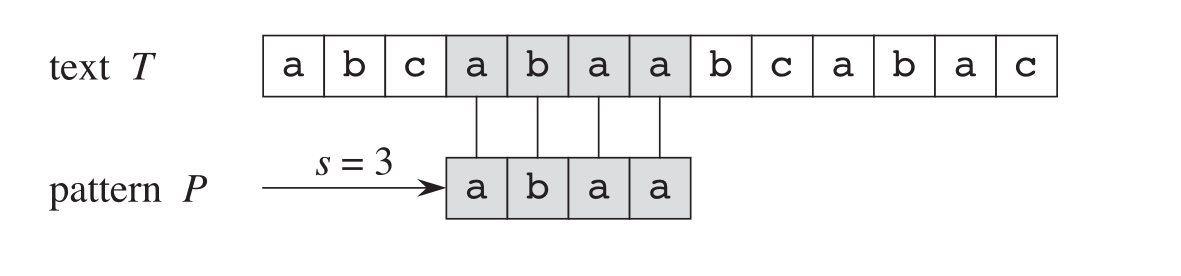
\includegraphics[width=400pt]{main--string-matching--notation-81a7.png}

\begin{itemize}
\item $\Sigma^{*}$ (Sigma-Stjerne) er sættet af alle endelige strenge der kan bliver lavet fra karaktererne i $\Sigma$. 
\item $\varepsilon$, den \textbf{tomme streng}, er strengen uden noget indhold. Den er også en del af $\Sigma^{*}$.
\item $|x|$ er længden af streng $x$. 
\item \textbf{Concatenation} af to strenge $x$ og $y$, skrevet $xy$ har længde $|x| + |y|$ og er karaktererne i $x$ efterfulgt af karaktererne i $y$.
\item \textbf{Præfiks} af streng $x$, denoted $w \sqsubset x$, gælder hvis $x = wy$ hvor $y \in \Sigma^{*}$, altså, $w$ er en del af streng $x$ i starten af strængen. $y$ er den resterende del af streng $x$, som ikke er $w$.
\item \textbf{Suffiks}: denoted $w \sqsupset x$ omvendt. 
\end{itemize}

\begin{lemma}[31.1 (Overlapping-suffix lemma) (Cormen)]
Suppose that $x,y$, and $z$ are strings such that $x \sqsupset z$ and $y \sqsupset z$. If $|x| \leq |y|$, then $x \sqsupset y$. If $|x| \geq |y|$, then $y \sqsupset x$. If $|x| = |y|$ then $x = y$.
\end{lemma}

\begin{proof}
  Se Figur ~\ref{fig:overlappingsuffix}
\end{proof}

\begin{figure}[ht]
  \centering
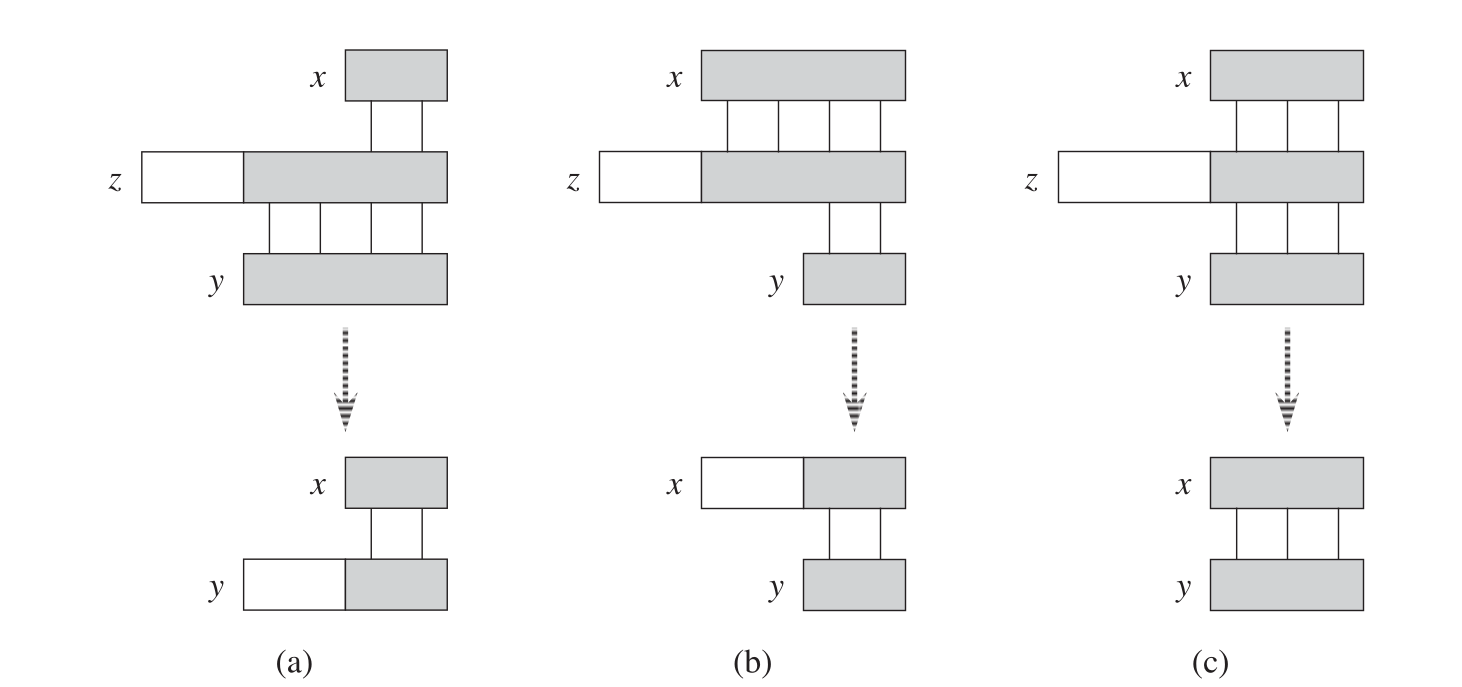
\includegraphics[width=400pt]{main--string-matching--notation-1e22.png}
  \caption{\label{fig:overlappingsuffix} Vi antager at $x \sqsupset z$ og $y \sqsupset z$. De tre dele af figuren illustrerer de tre cases af lemmaet. \textbf{(a)} Hvis $|x| \leq |y|$, så $x \sqsupset y$. \textbf{(b)} Hvis $|x| \geq |y|$, så $y \sqsupset x$. \textbf{(c)} Hvis $|x| = |y|$, så er $x = y$.}
\end{figure}

Vi antager at tiden det tager for at finde ligheden mellem to strenge er $\Theta(t+1)$ hvor $t$ er størrelsen af den længste streng. $+1$, til hvis $t = 0$.



\subsubsection{Køretids Overview}

\begin{table}[h]
\begin{tabular}{|l|l|l|}
\hline
\textbf{Algorithm}          & \textbf{Preprocessing Time} & \textbf{Matching Time} \\ \hline
\textit{Naive}              & $0$                         & $O((n-m+1)m)$          \\ \hline
\textit{Rabin-Karp}         & $\Theta (m)$                & $O((n-m+1)m)$          \\ \hline
\textit{Finite Automaton}   & $O(m |\Sigma |)$            & $\Theta (n) $          \\ \hline
\textit{Knuth-Morris-Pratt} & $\Theta (m)$                & $\Theta (n)$           \\ \hline
\end{tabular}
\end{table}


\subsection{Naive Algoritme}
\label{subsec:naive}

\begin{itemize}
\item Hvad er den? 
\item Hvorfor er den dårlig? 
\item Hvad er worst-case? 
\end{itemize}


Den naive algoritme er virkelig det, naiv.
\textbf{Source Code}:

\begin{verbatim}
Naive-String-Matcher(T,P)
n = T.length
m = P.length
for s = 0 to n - m
    if P[1..m] == T[s+1..s+m]
        print "Pattern occurs with shift " s
\end{verbatim}

\subsubsection{Køretid}

Den er virkelig skrald. Køretiden er $O((n-m+1)m)$. Dens worst case sker hvis teksten er $a^{n}$ og mønsteret der ledes efter er $a^{n}$ (begge er mængder af $a$'er, på længde hhv. $m$ og $n$. I dette tilfælde finder den matches hver gnag, og der tager dermed $O(n^{2})$ tid.

Der er \textbf{ingen} preprocessing tid, da der ikke skal gøres noget før algoritmen kører.



\subsection{Rabin-Karp}
\label{subsec:rabinkarp}

\begin{itemize}
\item Hvad er hovedidéen? 
\item Hvorfor er den bedre end naive? 
\end{itemize}

Trods at Rabin-Karp har en worst-case køretid på $\Theta((n-m+1)m)$ er dens gennemsnitlige køretid bedre.

Algoritmen konverterer bogstaverne til tal, i radix-$d$ notation, hvor $d$ er størrelsen på alfabetet, $|\Sigma|$.

I følgende eksempler vil vi gå ud fra at $d = 10$, og $\Sigma = \{0, 1, \ldots, 9\}$. Husk at $P[1..m]$ er mønsteret vi leder efter. Ved rabin-karp skelner vi mellem $P[1..m]$ og $p$, hvor $p$ er dets decimalværdi. Dvs., hvis $P[1..m] = 1372$, så er $p = 1372$ i decimalværdi. Eksemplet virker forsimplet idet vores alfabet også er tal, men tænk hvis alfabetet var $\Sigma = \{a, b, ... j\}$, i dette tilfælde ville $p$ ikke være ændret, men $P[1..m] = acgb$. Ydermere er teksten $T[1..n]$'s decimal counterpat $t_{s}$. Den bliver udregnet på samme måde. Hvis $t_{s} = p$ så $T[s+1..s+m] = P[1..m]$.

Vi vil gerne have en måde hvorpå vi kan lave alfabetet om til tal, som vi kan regne på. Hvis vi kan konverterer mønsteret $P[1..m]$ til $p$ på $\Theta(m)$ tid, så kan vi konvertere $t_{s}$ på $\Theta(n-m+1)$ tid. Til at gøre dette bruger vi \textbf{Horner's Rule}, som er meget vigtig at kende, se Definition ~\ref{def:horner}.

\begin{definition}[Horner's Rule]
  \label{def:horner}
  Horner's Rule er en regel hvorpå du hurtigt (specielt for computere) kan udregne decimaltal. Dette gør du ved at tage det sidste tal der skal udregnes først, derefter tager du tallet på 10'ernes plads, ganger det med $10^{1}$, etc. indtil du er ved $d$'ende plads, og ganger det med $10^{d}$\footnote{Dette gælder kun i base-10. Rabin-karp kører i base-b. Konverter dette til $b^{d}$}. Se følgende billede.


    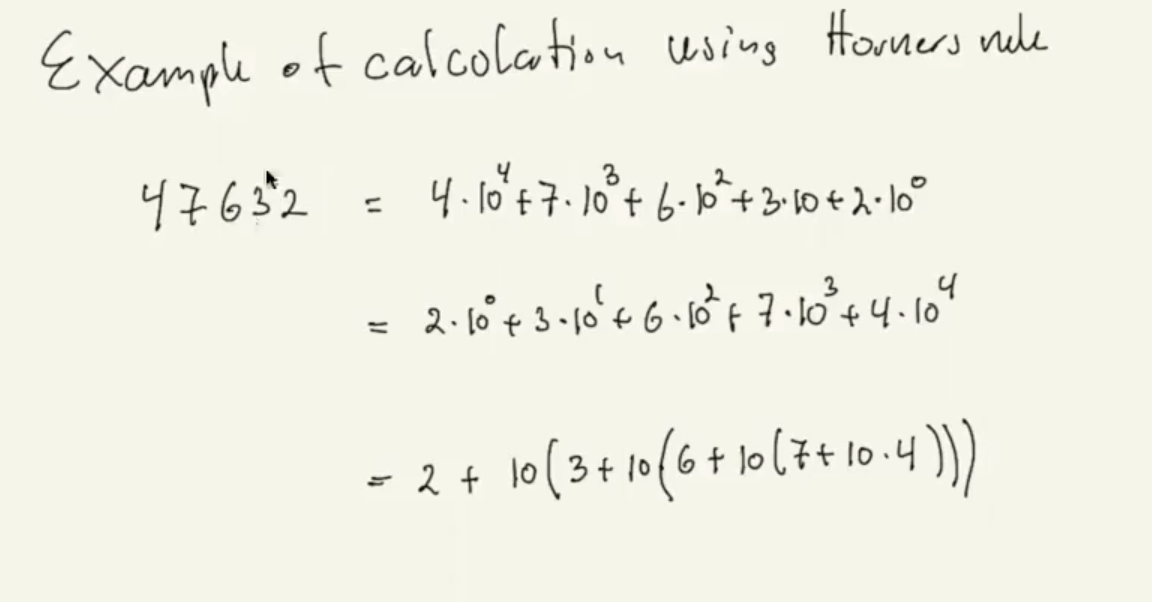
\includegraphics[width=300pt]{../Question8/main--the-naive-string-matching-algorithm--rabin-karp-c553.png} 
\end{definition}

Noget af det smarteste med Horner's Rule, er at, når du går til næste værdi, så kan du udregne det hurtigt uden at tage det hele om igen. Dette giver køretid $\Theta(n-m)$:

\[ t_{s+1} = 10(t_{s} - 10^{m-1}T[s+1]) + T[s+m+1] \]


\begin{forklaring}
\textit{Skip dette hvis du ikke har meget tid.} $10^{m-1} \cdot T[s+1]$ fjerner det højeste ciffer. Ved at gange det med 10 skifter du tallet til venstre med en cifferposition. Ved at tilføje $T[s+m+1]$ får du det nye, laveste ciffer. 
\end{forklaring}

\textbf{Problem!} $p$ og $t_{s}$ er muligvis for storre til at de kan være i et computer \texttt{word}. Hvis dette er tilfældet, og $P$ indeholder $m$ karakterer, så tager vi tallet \textbf{modulo }$q$. $p \mod q$ bliver udregnet på $\Theta(m)$ tid (størrelsen af $p$.) Alle $t_{s}$ værdier i $\Theta(n-m+1)$ tid.

\textbf{Hvilken $q$ skal vi dog vælge?} Simpelt! Vælg et primtal således der er plads til $10q$  i én computer \texttt{word}. Derefter kan vi udføre alle udregninger simpelt. Ved at bruge modulo-udregning, ændrer Horner's udregning sig til at blive: $t_{s+1} = (d(t_{s} - T[s+1]h) + T[s+m+1]) \mod q$, hvor $h \equiv d^{m-1} (\mod q)$ er værdien af ciffret $1$ i højeste position. 

\textbf{Problem igen!} Hvad hvis $p \equiv t_{s}$, men $P[1..m] \neq T[s+1..n-m]$? Altså, tallene er ens, men de er strengene ikke grundet modulo? Dette kalder vi et \textbf{spurious hit}, og er pisse irriterende, men desværre end nødvendig onde. Derfor, når vi finder et \textbf{hit} om det er spurious eller ej, så tjekker vi også strengene. 

\begin{figure}[ht]
  \centering
  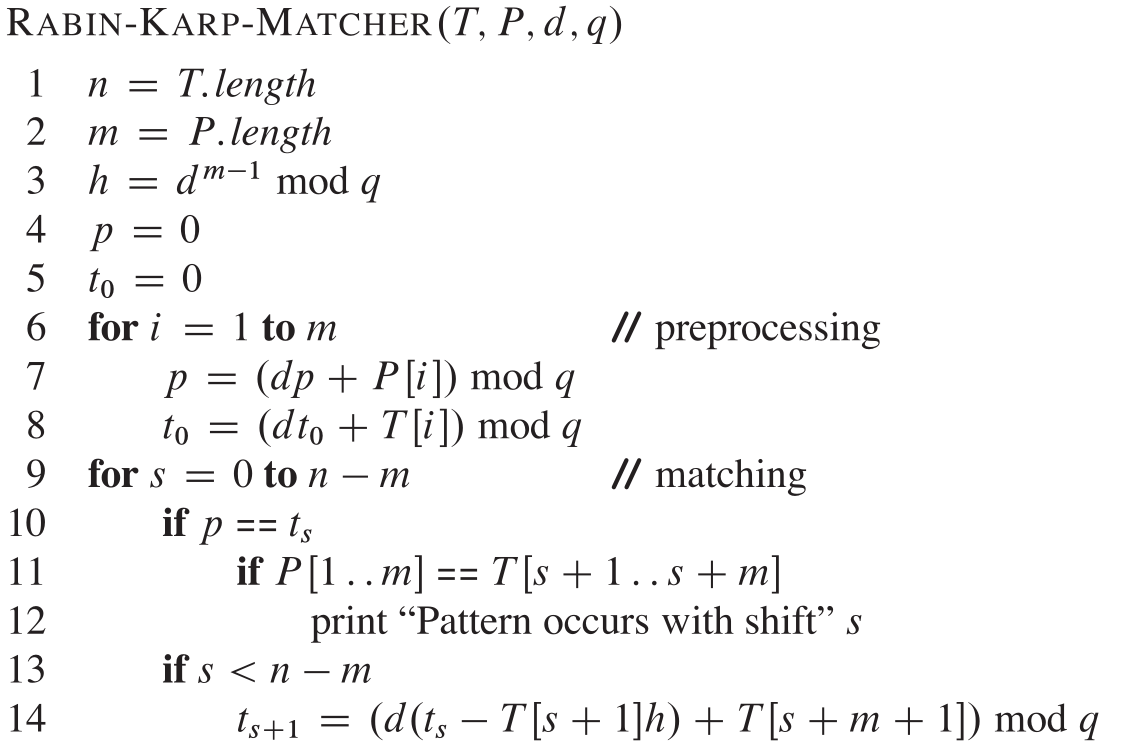
\includegraphics[width=400pt]{main--string-matching--rabin-karp-9fe7.png}
  \caption{\label{fig:rabinkarpalgorithm} Rabin Karp Algoritmen}
\end{figure}


Worst-case er i samme situation som ved den naive algoritme. Hvis teksten er en del a'er, og det samme med mønstret, så vil vi få en masse hits.



\subsubsection{Forventede antal hits}

Vi vil gerne finde det forventede antal hits. Vi antager at $\mod q$ agerer som en tilfældig mapping (funktion) fra alfabetet til heltal base $q$, altså $\Sigma^{*} \rightarrow \mathbb{Z}_{q}$. Ydermere antager vi at alle værdierne modulo $q$ er lige sandsynlige, i.e, $p(t_{s} \equiv p \mod q) = \frac{1}{q}$. Det vil sige at antallet af falske hits er $\frac{O(n)}{q} = O(\frac{n}{q}) $. Dette får vi fra antal af hvor mange der modulerer til samme værdi. Hvis der er 10 forskellige bogstaver, og vi er i base-3, så $\frac{10}{3} = 3.\overline{3}$ ca. tal der mapper til det samme.

Den forventede køretid bliver derfor $O(n) + O(m(v + \frac{n}{q}))$ hvor $v$ er antallet af korrekte hits, det's køretid er $O(1)$ og $q \geq m$. Dermed bliver den totale køretid $O(n+m) = O(n)$ da $n \geq m$.



\subsection{Finite Automaton Based}
\label{subsec:DFA}

\begin{itemize}
\item Hvordan laver man en DFA?
\end{itemize}

Jeg tænker \textbf{ikke} du behøver at forklare hvad en DFA er osv. Du får her en kort introduktion, som du bare kan springe over, givet at du forstår finite automata fint.

\subsection{Introduktion}
\label{subsec:DFAIntro}

Mange algoritmer bygger en Finite Automata (herfra forkortet som DFA), da den er utroligt hurtig til at finde matches. Hver karakter bliver kigget på præcis én gang, og bruger tid $O(1)$ per gang den bliver kigget på. Efter maskinen bliver bygget er matching tiden $\Theta(n)$. Dog kan tiden der bruges til at bygge maskinen være meget stor hvis $\Sigma$ er stort. 

\begin{definition}[Finite Automata]
  A \textbf{finite automaton} $M$, is a 5-tuple $(Q, q_{0}, A, \Sigma, \delta)$, where

  \begin{itemize}
  \item $Q$ is a finite set of \textbf{states}
  \item $q_{0} \in Q$ is the \textbf{start state}
  \item $A \subseteq Q$ is a disntinguished set of \textbf{accepting states},
  \item $\Sigma$ is a finite \textbf{input alphabet}, 
  \item $\delta$ is a function from $Q \times \Sigma$ into $Q$ called the \textbf{transition function} of  $M$.
  \end{itemize}
\end{definition}

Ved hvert state, læser maskinen et input, og går fra den state, $q$, til den næste defineret state, $\delta(q,a)$. Hvis $q$ er en del af $A$, og, efter strengen er blevet ``spist'', ender maskinen i $q \in A$, så er strengen ``accepteret'', ellers er den ikke. 

Ydermere bliver funktionen $\phi$ defineret som \textbf{Final-state funktion} fra $\Sigma^{*}$ til $Q$ således at $\phi(w)$ er den state som    $M$ ender op i, efter den scanner strengen $w$. Så, $M$ accepterer streng $w$ hvis \textbf{og kun hvis}, $\phi(w) \in A$.

\begin{equation}
  \label{eq:finalstatefunction}
\begin{split}
  \phi(\varepsilon) &= q_{0},\\
         \phi(wa) &= \delta(\phi(w),a) \; \; \text{for } w \in \Sigma^{*}, a \in \Sigma\\
\end{split}
\end{equation}


\subsection{Streng-matchende automat}
\label{subsec:stringmatchingautomata}


For at givet mønster $P$, vil vi lave en streng-matchende automat som preprocessing skridt før den bruges til at søge efter strengen.  Se figur~\ref{fig:stringmatchingautomata} for hvordan vi konsturerer automaten for mønstret $P = ababaca$. 

\begin{figure}[ht]
  \centering

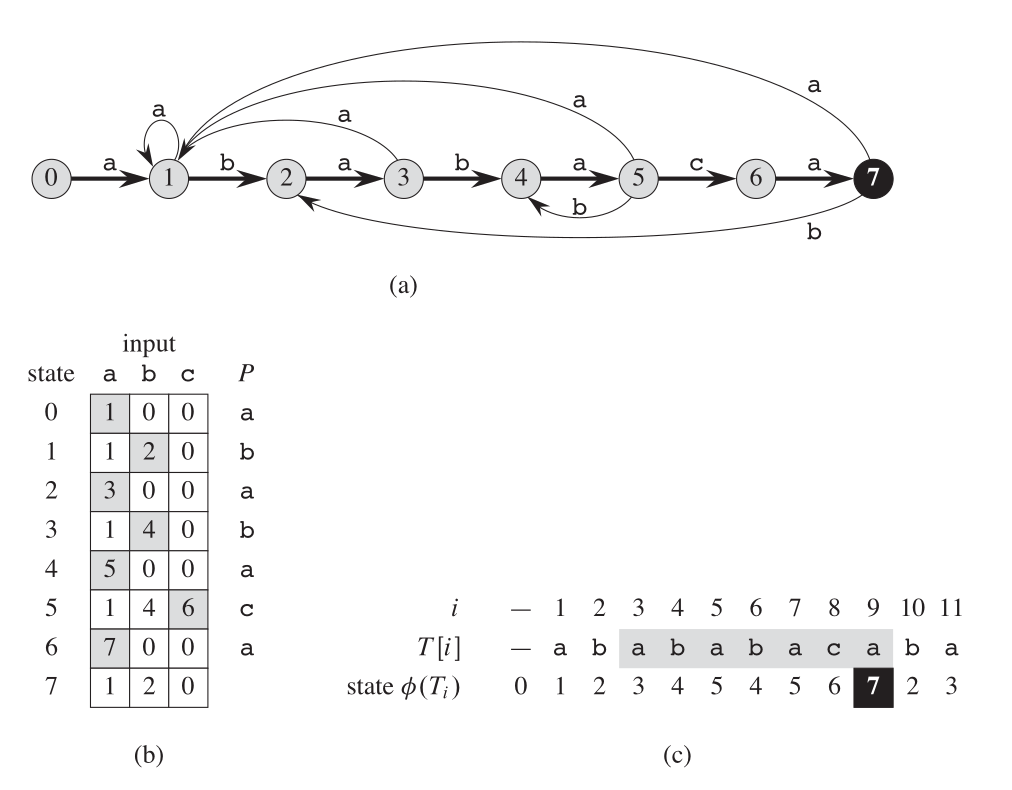
\includegraphics[width=400pt]{main--string-matching--streng-matchende-automat-6f23.png}  \caption{\label{fig:stringmatchingautomata} For mere information om figuren, se pp. 997 i Cormen}
\end{figure}


\begin{definition}[Suffiks Funktion]
  Givet et mønster $P[1..m]$, definerer vi funktionen $\sigma$, kaldet \textbf{suffiks funktion} korresponderende til $P$. Funktionen $\sigma$ mapper $\Sigma^{*}$ til $\{0,1, \ldots, m\}$, således at $\sigma(x)$ er længden af det længste præfix af $P$ som også er et suffiks af $x$:
  \[ \sigma(x) = \text{max}\{k : P_{k} \sqsupset x\} \]

  Suffiks Funktionen  er \textbf{well-defined} (hvert element mapper til noget), da $P_{0} = \varepsilon$ er et suffiks er hver streng. 
\end{definition}

\begin{example}[Eksempler på Suffiks Funktionen]

  Givet mønstret $P = ab$, har vi $\sigma(\varepsilon) = 0$, $\sigma(ccaca) = 1$ og $\sigma(ccab) = 2$.
  Givet mønstret med længde $m$ har vi $\sigma(x) = m$ hvis og kun hvis $P \sqsupset x$. Fra definitionen af suffiksfunktionen betyder $x \sqsupset y$ også at $\sigma(x) \leq \sigma(y)$.
\end{example}

Vi definerer en streng-matchende automat som korresponderende til et mønster $P[1..m]$ som følger:

\begin{itemize}
\item Sættet af states $Q$ er $\{0, 1, \ldots, m\}$. Start staten $q_{0}$, og staten $m$ er de eneste accepteret states. 
\item Transition function $\delta$ er defineret ved følgende ligning, for hver state $q$ og karakter $a$:

  \begin{equation}
    \label{32.4}
\delta(q,a) = \sigma(P_{q}a)
  \end{equation}
  
\end{itemize}

Det vil sige, at givet en karakter $a$, vil vi gå fra state $q$ til længden af det længste præfiks af $P$, som også er et suffiks af $x$. Så, altså, hvis $a$ får dig én længere, vil du også gå én state tilbage. Men, hvis du går tilbage til kun at være 2 inde, så er du tilbage på state 2. 

\begin{forklaring}[Yderligere forklaring]
  \label{forkl:yderligeredfa}
  Vi definerer $\delta(q,a) = \sigma(P_{q}a)$ fordi vi vil holde fast i det længste præfix af mønsteret $P$ der har matchet strengen $T$ indtil videre.

  Antag at $p = \phi (T_{i})$, så, efter at have læst $T_{i}$, så er automatonet i state $q$. Vi designer $\delta$ således at state $q$ fortæller os længden af det længste præfiks af $P$ der er en suffiks af $T_{i}$. Det vil sige, i state $q$, $P_{q} \sqsupset T_{i}$ og $q = \sigma(T_{i})$. Dette vil også sige at \textbf{hvis $q = m$, så har vi fundet et match!} Dermed, siden $\phi (T_{i})$ og $\sigma(T_{i})$ begge er lig $q$, ser vi at automaten holder følgende invariant:

  \begin{equation}
    \label{32.5}
\phi(T_{i}) = \sigma(T_{i})
  \end{equation}

  Dermed, hvis vi er i state $q$, og automaten læser karakter $T[i+1] = a$, så skal vores transition lede til det korresopnderende længste præfiks af $P$ som er et suffiks af $T_{i}a$. Den state er $\sigma(T_{i}a)$. 
  
Fordi $P_{q}$ er det længste præfiks af $P$ som er et suffiks af $T_{i}$, så er det længste præfiks af $P$ som er et suffiks af $T_{i}a$ ikke kun $\sigma(T_{i}a)$, men også $\delta(P_qa)$. (Dette bliver bevist senere)
\end{forklaring}

Der er to states vi skal kigge på, den første, $a = P[q+1]$, så er $\delta(q,a) = q+1$.
Den næste, $a \neq P[q+1]$, så skal vi finde et mindre præfiks af $P$ som også er et suffiks af $T_{i}$.

Lad os kigge på et eksempel. Streng-matching automaten fra Figur~\ref{fig:stringmatchingautomata} har $\delta(5,c) = 6$, som så er first case, hvor vi bare går videre. Et sekmepl på second case er $\delta(5, b) = 4$. Vi laver denne transition fordi, hvis automaten læser et $b$ når $q = 5$, så $P_{q}b = ababab$, og det længste præfiks af $P$ som også er et suffiks af $ababab$ er $P_{4} = abab$.

Følgende er algoritmen for at lave en finite automata til streng-matching. Sættet af states $Q = \{0, 1, \ldots, m\}$, start staten $q_{0} = 0$, den eneste accepting state er $m$, ${m} \in A$.


\begin{figure}[ht]
  \centering
  \begin{verbatim}
Finite-Automaton-Matcher(T, d, m):

n = T.length
q = 0
for i = 1 to n
    q = d(q, T[i])
    if q == m
        print "Pattern occurs with shift" i - m
\end{verbatim}
  \caption{\label{fig:dfa-algorithm} }
\end{figure}

Transition function er som beskrevet tidligere. Hvis dette ikke er klart, se Forklaring \ref{forkl:yderligeredfa}.

Det er her nemt at se at køretiden på en tekst-streng af længde $n$ er $\Theta(n)$.
Før vi viser pre-processing tid, kigger vi på et bevis for at algoritmen kører som forventet.


\begin{figure}[ht]
  \centering
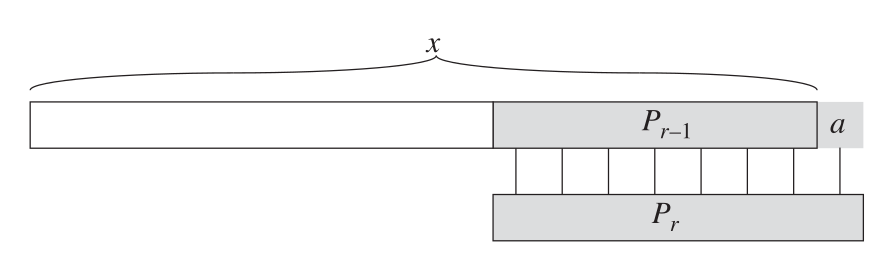
\includegraphics[width=300pt]{32.8.png}  
  \caption{\label{fig:32.8} En illustration til beviset af Lemma~\ref{lemma:suffixfunctioninequality}. FIguren viser $r \leq \delta(x) + 1$, hvor $r = \delta(xa)$}
\end{figure}


\begin{lemma}[Suffix-Function Inequality]
  \label{lemma:suffixfunctioninequality}
  For hver streng $x$ og karakter $a$, har vi at $\sigma(xa) \leq \sigma(x) + 1$.
\end{lemma}

\begin{proof}
Se Figur~\ref{fig:32.8}. Hvis $r = 0$, så $\sigma(xa) = r \leq \delta(x) + 1$ er trivielt løst, da $\sigma(x)$ er nonnegativt. Antag at $r > 0$, så $P_{r} \sqsupset xa$ per definition af $\sigma$. Dermed, $P_{r-1} \sqsupset x$, ved at fjerne $a$ fra enden af $P_{r}$ og fra enden af $xa$. Dermed $r-1 \leq \sigma(x)$, siden $\sigma(x)$ er det største $k$ således $P_{k} \sqsupset x$, og således $\sigma(xa) = r \leq \sigma(x) + 1$
\end{proof}

\begin{figure}[ht]
  \centering
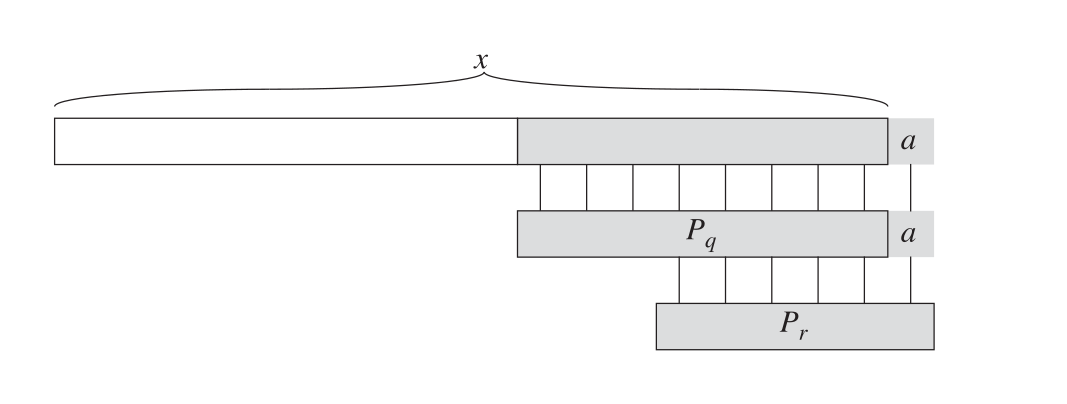
\includegraphics[width=300pt]{32.9.png}
  \caption{\label{fig:32.3} Illustration af beviset for Lemma~\ref{lemma:32.3}. Figuren fiser at $r = \delta(P_{q}a)$, hvor $q = \sigma(x)$ og $r = \sigma(xa)$}
\end{figure}


\begin{lemma}[Suffix-Function Recursion Lemma]
\label{lemma:32.3}
For enhver streng $x$ og karakter $a$, hvis $q = \sigma(x)$, så $\sigma(xa) = \sigma(P_{q}a)$.
\end{lemma}

\begin{proof}
Vi ved fra definitionen af $\sigma$ at $P_{q} \sqsupset x$. Som vist i figur~\ref{fig:32.3}, har vi også $P_{q}a \sqsupset xa$. Hvis $r = \sigma(xa)$, så $P_r \sqsupset xa$ og, gennem Lemma~\ref{lemma:suffixfunctioninequality}, $r \leq q + 1$. Dermed har vi at $|P_{r}| = r \leq q + 1 = |P_{q}a|$. Derfor, $r \leq \sigma(P_{q}a)$, dermed $\sigma(xa) \leq \sigma(P_qa)$. Vi har dog også $\sigma (P_{q}a) \leq \sigma(xa)$, siden $P_{q}a \sqsupset xa$. Dermed $\sigma(xa) = \sigma(P_{q}a)$
\end{proof}

Tid til det vigtigste skridt. Vi skal vise at automaten vedligeholder invarianten i ligning \ref{32.4}.

\begin{theorem}
  \label{the:32.4}
  If $\phi$ is the final-state function of a string-matching automaton for a given pattern $P$ and $T[1..n]$ is an input text for the automaton, then
  $\phi(T_{i}) = \sigma(T_{i})$
  for $i = 0, 1, \ldots, n$.
\end{theorem}

\begin{proof}
  Vi beviser gennem induktion på $i$.

 Ved $i = 0$ er teoremet sandt, da $T_{0} = \varepsilon$ dermed $\phi(T_{0}) = 0 = \sigma(T_{0})$.
\end{proof}

Vi antager nu at $\phi (T_{i}) = \sigma(T_{i}) $ og beviser at $\phi(T_{i+1}) = \sigma(T_{i+1})$.
Lad $q$ være $\phi(T_{i})$, og lad $a$ være $T[i+1]$.
Så:

\begin{equation*}
  \begin{split}
    \phi(T_{i+1}) &= \phi T(_{i}) \; \text{(fra definition på} $T_{i+1}$ \text{ og } \text{a})\\
               &= \delta(\phi (T_{i}), a) \; \text{(fra definitionen på} \phi \text{)}\\
               &= \delta(q,a) \; \text{(af defintiion på q)}\\
               &= \sigma(P_{q}a) \; \text{(fra definitionen tidligere )}\\
               &= \sigma(T_{i}a)\\
                 &= \sigma(T_{i+1}) \\
  \end{split}
\end{equation*}


\subsection{Find Transition Function}

Vi vil gerne finde transition funktion. Vi har allerede defineret den tidligere, men vi vil have en algoritmisk metode hvorpå vi kan gøre det.


\begin{figure}[ht]
  \centering
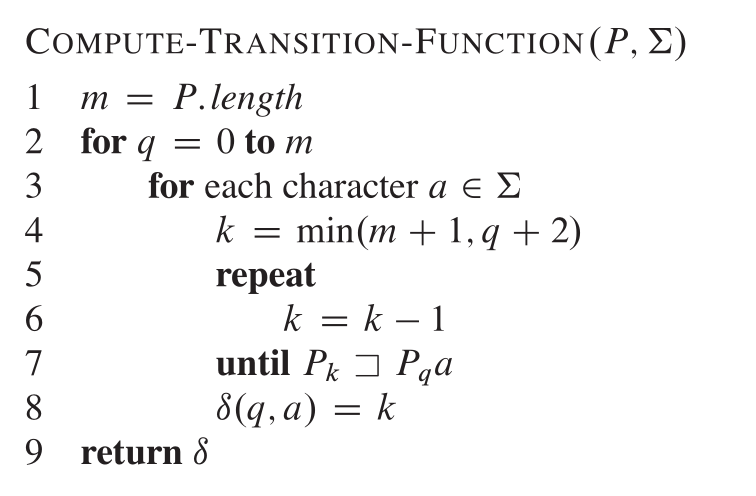
\includegraphics[width=250pt]{compute-transition-function.png}
  \caption{\label{fig:compute-transition-function} Algoritmen for at finde transition function på.}
\end{figure}

Køretiden på algoritmen er $O(m^{3}|\Sigma|)$.



\section{Flows}
\label{sec:flows}

\section{Min-Cut}
\label{sec:mincut}





\end{document}
